$if(has-frontmatter)$
\frontmatter
$endif$
% ---------- Sampul ----------
\begin{titlepage}
\thispagestyle{empty}
\begin{tikzpicture}[remember picture, overlay]
  \node[anchor=south, inner sep=0pt, opacity=0.18] at (current page.south)
    {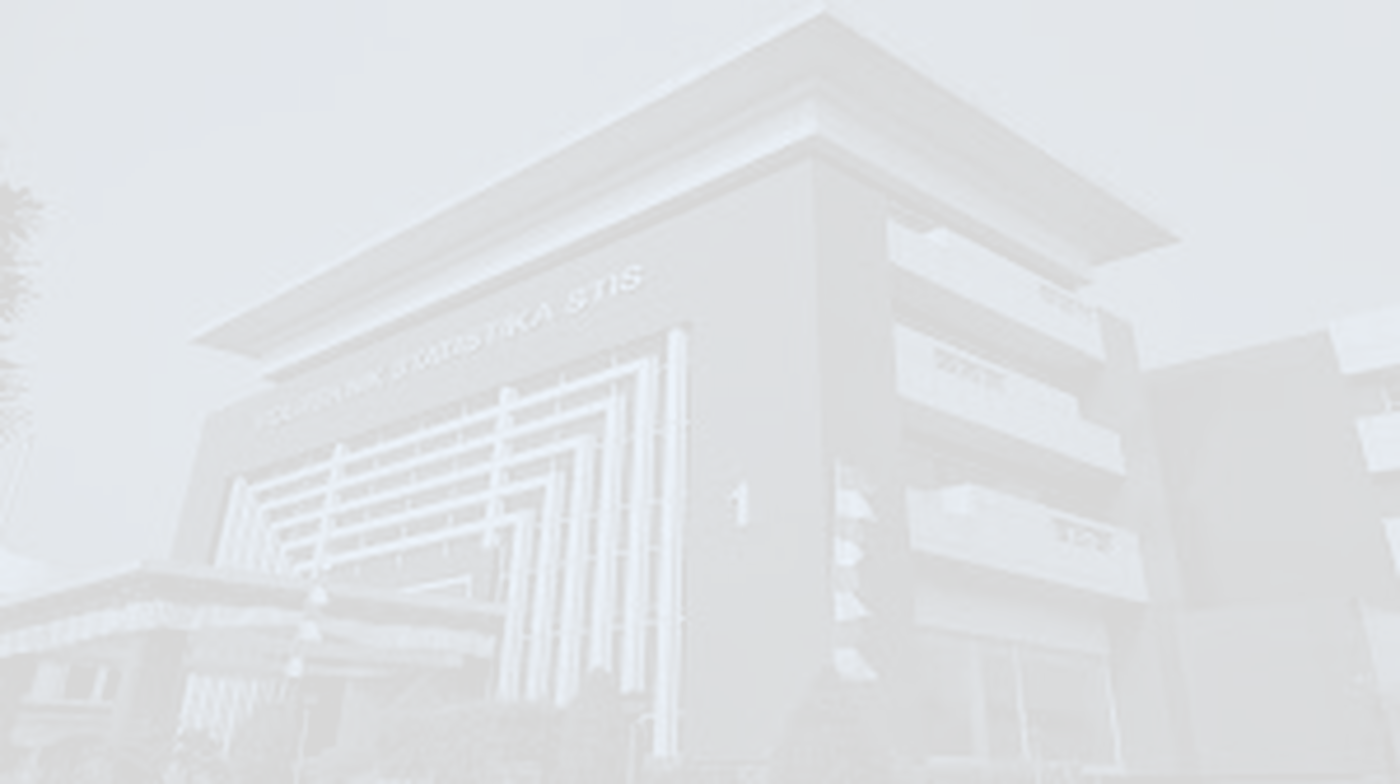
\includegraphics[width=\paperwidth]{gambar/gedung_bg.png}};
  \fill[bpsnavy] (current page.north west) -- ++(0,-9.2cm) --
        ($$(current page.north east)+(0,-6.4cm)$$) -- (current page.north east) -- cycle;
  \fill[bpsbiru] ($$(current page.north west)+(0,-9.2cm)$$) -- ++(0,-0.9cm) --
        ($$(current page.north east)+(0,-7.3cm)$$) -- ($$(current page.north east)+(0,-6.4cm)$$) -- cycle;
  \fill[bpsoranye] ($$(current page.north west)+(0,-10.1cm)$$) -- ++(0,-0.25cm) --
        ($$(current page.north east)+(0,-7.55cm)$$) -- ($$(current page.north east)+(0,-7.3cm)$$) -- cycle;
  \node[anchor=north west, inner sep=0pt] at ($$(current page.north west)+(2.2cm,-1.8cm)$$)
    {
\includegraphics[height=2.2cm]{gambar/logo_stis.png}};
  \node[anchor=north west, text=white, align=left, font=\sffamily] at
    ($$(current page.north west)+(5.2cm,-2.0cm)$$)
    {\Large\bfseries POLITEKNIK STATISTIKA STIS\\[4pt]\normalsize Buku Pedoman Aplikasi};
  \node[anchor=north west, text width=15cm, align=left, font=\sffamily] at
    ($$(current page.north west)+(2.2cm,-12.3cm)$$)
    {{\color{bpsoranye}\large\bfseries BUKU PEDOMAN}\\[10pt]
     {\color{bpsnavy}\fontsize{28}{34}\selectfont\bfseries\hyphenpenalty=10000\exhyphenpenalty=10000 $title$}\\[14pt]
     {\color{bpsbiru}\Large\parbox[t]{15cm}{\raggedright\hyphenpenalty=10000\exhyphenpenalty=10000 $subtitle$}}};
  \fill[bpsnavy] ($$(current page.south west)+(0,3.4cm)$$) rectangle (current page.south east);
  \fill[bpsoranye] ($$(current page.south west)+(0,3.4cm)$$) rectangle
        ($$(current page.south east)+(0,3.55cm)$$);
  \node[anchor=west, text=white, align=left, font=\sffamily] at
    ($$(current page.south west)+(2.2cm,1.75cm)$$)
    {\large\bfseries $for(author)$$author$$sep$, $endfor$\\[3pt]
     \normalsize Untuk paket \texttt{modulstis} versi \versimodulstis{} \quad$$\cdot$$\quad $date$};
\end{tikzpicture}
\end{titlepage}

% ---------- Halaman hak cipta ----------
\thispagestyle{empty}
\vspace*{\fill}
{\small\color{abuteks}
\textbf{\color{bpsnavy}Buku Pedoman $title$}\\
$subtitle$\\[8pt]
\begin{tabular}{@{}ll@{}}
Jenis ciptaan & Program komputer (paket R)\\
Nama program & \texttt{modulstis}, versi \versimodulstis{}\\
Pencipta & $for(author)$$author$$sep$, $endfor$\\
Institusi & Politeknik Statistika STIS, Jakarta\\
Bahasa pemrograman & R\\
Lisensi & MIT\\
Kode sumber & \url{https://github.com/madsyair/modulstis}\\
Diperbarui & $date$\\
\end{tabular}\\[10pt]
Seluruh contoh kode dalam buku ini dijalankan ketika buku dibangun, sehingga keluaran yang
tercetak adalah keluaran aplikasi yang sebenarnya. Kode sumber di lampiran dibaca langsung dari
berkas paket versi yang sama. Gambar antarmuka RStudio adalah tangkapan layar RStudio Server
2026.10.1.\par}
\clearpage
